%% The first command in your LaTeX source must be the \documentclass command.
%%
%% Options:
%% twocolumn : Two column layout.
%% hf: enable header and footer.
\documentclass[
twocolumn,
% hf,
]{ceurart}

%%
%% One can fix some overfulls
\sloppy

%%
%% Minted listings support 
%% Need pygment <http://pygments.org/> <http://pypi.python.org/pypi/Pygments>
\usepackage{listings}
\usepackage{bm}
\usepackage{url}
\usepackage{array,multirow,graphicx}
\usepackage{float}

%% auto break lines
\lstset{breaklines=true}

%%
%% end of the preamble, start of the body of the document source.
\begin{document}

%%
%% Rights management information.
%% CC-BY is default license.
\copyrightyear{2022}
\copyrightclause{Copyright for this paper by its authors.
  Use permitted under Creative Commons License Attribution 4.0
  International (CC BY 4.0).}

%%
%% This command is for the conference information
\conference{COMHUM 2022: Workshop on Computational Methods in the Humanities,
  June 9--10, 2022, Lausanne, Switzerland}

%%
%% The "title" command^
\title{Refining character relationships using embeddings of textual units : a case study on Les Misérables}

%%
%% The "author" command and its associated commands are used to define
%% the authors and their affiliations.
\author[1]{Guillaume Guex}[%s
orcid=0000-0003-1001-9525,
email=guillaume.guex@unil.ch]
\address[1]{Departement of Language and Information Sciences, University of Lausanne, Switzerland}

%%
%% The abstract is a short summary of the work to be presented in the
%% article.
\begin{abstract}
  A clear and well-documented \LaTeX{} document is presented as an
  article formatted for publication by CEUR-WS in a conference
  proceedings. Based on the ``ceurart'' document class, this article
  presents and explains many of the common variations, as well as many
  of the formatting elements an author may use in the preparation of
  the documentation of their work.
\end{abstract}

%%
%% Keywords. The author(s) should pick words that accurately describe
%% the work being presented. Separate the keywords with commas.
\begin{keywords}
  LaTeX class \sep
  paper template \sep
  paper formatting \sep
  CEUR-WS
\end{keywords}

%%
%% This command processes the author and affiliation and title
%% information and builds the first part of the formatted document.
\maketitle

\section{Introduction}

Distant reading tools allow researchers, from various fields, to quickly gain knowledge on textual corpora without actually reading them. Purposes of these methods are various, but can be mainly categorized into two groups: in the first case, these methods are used in order to tag, classify, or summary large quantities of texts, in order to quickly structure information or to deliver a speech over the whole studied corpus. Methods in this case rely heavily on Big Data and make an extensive use of Machine Learning algorithms. In the second case, researchers use these methods to underline hidden structures in a particular text, helping them to refine their understanding of it and reinforce stated hypotheses. Methods in this setting can also rely on Machine Learning, but must typically be build with more caution and attention to details: corpus are smaller, analyses are closer to the work, and methods must be more transparent in order to appropriately interpret results.

Automatic extraction and analysis of \emph{character networks} from literacy works typically belong in the latter group. These methods aim at representing various interactions occurring between fictional characters found in a textual narrative with a graph, thus showing explicitly the hidden structure of character relationships constructed by the author. This structure might allow to find hidden patterns within a book, which can highlight a particular genre or style.

\section{Methodology}


When building character networks from a textual narrative, the most widespread method consists in dividing the studied work into $n$ textual units $u_1, \ldots, u_n$, which can be, e.g., sentences, paragraphs, or chapters, and then counting characters co-occurrences in these units. Usually, the text constituting these units is discarded and the resulting network displays edges which roughly represent an aggregated number of interactions between characters. However, by doing so, the aggregation occurs on various type of interactions and will give little information about the type of relationship which exist between characters. In this paper, we propose a data organization leading to various methods which takes into consideration the text contained in the unit, helping to refine understanding of characters and their relationships.

\subsection{Data organization}

In this article, the data representation for a textual narrative, divided in $n$ textual units $u_1, \ldots, u_n$, is made through two tables. The first one is well known in the field of textual analysis, and consists in the $(n \times v)$ contingency table $\mathbf{N}$, as represented by Table 1, where $v$ is the vocabulary size. In this table, each row represents an unit, each column a word, and cells $n_{ij}$ counts the number of times the word $i$ appears in the unit. Using this table typically denotes a \emph{Bag-of-Words} approach in our analyses.

\begin{table}[h]
	\scriptsize
	\begin{tabular}{|c||c|c|c|c|c|c|}
		\hline
		& aller & allumer & apercevoir & bas & bon & ... \\
		\hline
		\hline 
		$u_{101}$ & 23 & 2 & 6 & 11 & 6 & ... \\
		\hline
		$u_{102}$ & 12 & 1 & 0 & 3 & 9 & ... \\
		\hline
		$u_{103}$ & 10 & 0 & 5 & 1 & 5 & ... \\
		\hline
		$u_{104}$ & 0 & 0 & 1 & 0 & 0 & ... \\
		\hline
	\end{tabular}
	\label{cont_table}
	\caption{A snippet of the contingency table $\mathbf{N}$ extracted from \emph{les Misérables}. Rows are chapters, columns are words in the vocabulary, and cell $n_{ij}$ counts the number of time word $j$ appear in chapter $i$.}
\end{table}

The second table, denoted by $\mathbf{O}$, has a size of $(n \times p)$ where $p$ is the number of \emph{entities} found in the narrative and cells $o_{ij}$ indicates the presence, or the count for a weighted version, of entity $j$ in unit $i$. An entity, in the context of this article, can be loosely defined in order to be flexible for various types of narrative or analyses, but can roughly be seen as a recurring narrative object, which can contain one or more characters. For example, it can be a character, pair of characters (or even triplet, quadruplet, etc.), an oriented character interaction (e.g. a dialog), or even a particular recurring event containing multiple characters (e.g. a meeting). In this article, we mostly consider character and pair of characters as entities, as shown in Table 2. Note that we consider that a character or a pair of characters are present in the unit if character names (or aliases) are detected above a fixed threshold. A weighted version of this table, where $o_{ij}$ contain the number of occurrences of the entity $j$ in the unit $i$, is also possible and the theory will be written accordingly.

\begin{table}[h]
	\scriptsize
	\begin{tabular}{|c||c|c|c|c|}
		\hline
		& Cosette & Thénardier & Valjean & ... \\
		\hline
		\hline 
		$u_{101}$ & 1 & 1 & 0 & ... \\
		\hline
		$u_{102}$ & 1 & 1 & 0 & ... \\
		\hline
		$u_{103}$ & 1 & 1 & 0 & ... \\
		\hline
		$u_{104}$ & 1 & 0 & 1 & ... \\
		\hline
	\end{tabular}
	\begin{tabular}{|c||c|c|c|c|}
		\hline
		& ... & Cosette-Thénardier & Cosette-Valjean & ... \\
		\hline
		\hline 
		$u_{101}$  	& ... & 1 & 0 &  ... \\
		\hline
		$u_{102}$ 	& ... & 1 & 0 & ... \\
		\hline
		$u_{103}$  	& ... & 1 & 0 & ... \\
		\hline
		$u_{104}$ 	& ... & 0 & 1 & ... \\
		\hline
	\end{tabular}
	\label{occ_table}
	\caption{A snippet of the entities table $\mathbf{O}$ extracted from \emph{les Misérables}. Rows are chapters, columns are characters (top) and character-pairs (bottom), and cell $o_{ij}$ denotes if $j$ appear in chapter $i$.}
\end{table}

This data organization already gives an orientation to the subsequent analyses and should be kept in mind of the practitioner. Textual unit are now considered as \emph{individuals} (in the statistical terminology), defined by their \emph{variables} contained in the different columns of both tables. Moreover, subsequent analyses are oriented in searching how the entity table $\mathbf{O}$ has an influence over the contingency table $\mathbf{N}$, i.e. searching which words are over-represented or under-represented knowing entities in the unit. While authors use characters in order to build the narrative, we, to a certain extent, work backward: we are searching how character appearances and interactions in the textual unit act on her/his choice of words. If the extraction method permits it, a practitioner should include all entities which she/he desire to study. Here, for example, the choice to include character-pairs along with characters is motivated by the fact that we are interested in studying character relationships. A character-pair can roughly be seen as an interaction between two characters, and this interaction should be considered as an object of its own: the presence of this interaction in a unit do not result in having a mixture of words used for each character, and rather give a particular flavor to the unit. 

This data organization also highlight the importance of choosing a proper size for the units. These units should be large enough to contain enough words in order the properly capture the textual specificity of each unit, but not too large, as each unit should ideally captures particularities about one of the entity. Unfortunately, it is impossible to define an ideal size for all types of analysis and this size should be balanced regarding the level of analysis, the text size, the selected entities, and previous knowledge of the studied work.

The use of a contingency table $\mathbf{N}$ to represent the textual resource present in the units denotes a \emph{Bag-of-Words} approach. Using this approach loses the information relative to the order of words in the units, but permits to transform a chain of characters, improper to statistical analyses, into a contingency table, a well studied mathematical object which allows the use of various kind of statistical methods. The next section shows two methods of analysis based on this table.

\subsection{Embedding of textual units}
\label{unit_embeddings}

Various methods can be performed on the contingency table $\mathbf{N}$ in order to extract information from it, such as Sentiment Analysis (REF), Textometry (REF), or even Deep Learning methods (REF?). Here, we make to choice to extract a lower dimensional, numeric representation of each units, in other words, an \emph{embedding of textual units}. \\
In section \ref{entity_embeddings}, these vectors of textual units are used as anchor points in order to also embed entities into the same space. Therefore, it is crucial that an interpretation about the directions, or the regions, of this embedding is possible in order to properly extract information about the localization of entity vectors (the relative position of these entity vectors among themselves is insufficient). For that reason, we focus on embeddings of textual units which also contain \emph{vectors of words}: by examining the positions of entities relatively to word vectors, these entities can be characterized.

We propose here two embeddings verifying this condition: Section \ref{ca_method} describes \emph{Correspondence Analysis (CA)} and section \ref{wv_method} focuses on \emph{Pre-trained Word Vectors (WV)}. 

\subsubsection{Correspondence Analysis (CA)}
\label{ca_method}

Using Correspondence Analysis in order to analyze textual resources has a long tradition in literature (REF). It has the advantage to naturally provide an embedding space, the factorial map, where units are placed alongside word vectors, allowing to analyze or represent the different units in terms of word frequency profiles. Moreover, units and words placement in the embedding space have a direct interpretation in terms of chi2 distance between profiles, which is desirable when interpreting results.

By performing a Correspondence Analysis on table $\mathbf{N}$, we directly get $n$ vectors $\mathbf{x}_1, \ldots, \mathbf{x}_n$ corresponding to units (rows) and $v$ vectors $\mathbf{w}_1, \ldots, \mathbf{w}_v$ corresponding to words (columns). Each of these vectors has a size of $\min(n, v) - 1$, which will generally be $n - 1$. For a detailed computation of quantities in CA, see Appendix \ref{ca_details}. 

The association between a particular unit $i$ and a word $j$ is expressed through the scalar product between their vectors $s_{ij} := \mathbf{x}^\top_i \mathbf{w}_j$, which act as a similarity measure. A positive (resp. negative) similarity denotes a over-representation (resp. under-representation) of the word $j$ in $i$, which permit to find lists of words characterizing the different units. Observe that in this article, this similarity is rather computed between word and entity vectors, as defined in section \ref{entity_embeddings}, as they lie in the same space as unit vectors. 

Using CA to embedded units however comes with limitations. First, note that vectors $\mathbf{x}_1, \ldots, \mathbf{x}_n$ obtained from CA reflect textual unit profile (in terms of words) regarding the mean profile. This analysis is thus \emph{contrastive}: it highlights unit variations among the studied text. This could becomes problematic in order to study a dataset containing multiple corpora: units belonging to the same text will have a greater chance to be close from each other, and the displayed variance might be largely composed by differences of style between the different works. Another limitation with this approach is that the words helping the interpretation of units (and entities) are contained in the studied text. Approaches requiring to study the position of units and entities relatively to a predefined list of words (e.g., friends, enemies, family) might therefore be impossible if these words do not appear in the text.

\subsubsection{Pre-trained Word Vectors (WV)}
\label{wv_method}

Pre-trained word vectors, based on methods such as Word2Vec (REF), Glove (REF), or fastText (REF), have recently received great attention from various fields (REFS). They are generally obtained through a training on a very large corpora, such as Wikipedia (REF) or Common Crawl (REF), and the resulting embedding contains a large quantity of word vectors. As shown by multiple studies (REF), these vectors are placed in order to reflect semantic and syntactic similarities between words, and are used in mutliple applications (REF). 

There exists various ways to use these pre-trained word vectors in order to find vectors for a \emph{group of words}, such as sentences (REF), paragraphs (REF), or documents (REF). These vectors are often used to apply a classification or clustering algorithm on the newly embedded objects (REF), or to query information (REF). These methods often use the frequencies of words found in the objects, i.e. a table similar to $\mathbf{N}$, but apply various weighting scheme and normalization in order to reduce the effects of frequent words and to align vectors. In the present article, we use a recent methodology proposed in (REF) as it is compatible with multiple unit sizes and gives state-of-the-art results in various tasks. 

Textual units vectors $\mathbf{x}_1, \ldots, \mathbf{x}_n$ are obtained through the table $\mathbf{N}$ and with the method detailed in Appendix \ref{wv_details}. The main way to interpret units with this method is to use the cosine similarity between its corresponding vector $\mathbf{x}_i$ and every word-vectors $\mathbf{w}_j$, as defined by $s_{ij} := \frac{\mathbf{x}_i^\top \mathbf{w}_j}{\sqrt{\mathbf{x}_i^\top \mathbf{x}_i \mathbf{w}_j^\top \mathbf{w}_j}}$. The cosine similarity also permits to compare units between themselves.

With the pre-trained word vector method, the unit vectors $\mathbf{x}_1, \ldots, \mathbf{x}_n$ (and entity vectors in section \ref{entity_embeddings}) lie in an \emph{absolute space} defined by the used word vectors. Comparison between different texts are therefore more pertinent in this space and comparison with words absent from the corpus can be made. However, it is possible that all units from a given text, if the author style is particularly marked, are located in the same region of the space. In this case, the list of most associated word-vectors might be similar for every unit, and the analysis might not give usable results. This effect is fortunately limited by the centration of unit-vectors which occurs in the method describe in Appendix \ref{wv_details}.

\subsection{Entity embeddings}
\label{entity_embeddings}

The main goal of this article is not to analyze units, but rather the entities, i.e. the $p$ columns of table $\mathbf{O}$. While we used the table $\mathbf{N}$ to build our embeddings of units, we now use the table $\mathbf{O}$ in order to build the entity vectors $\mathbf{y}_1, \ldots, \mathbf{y}_p$ which lie in the same space as units. 

Two propositions of method are made: the \emph{centroids} method (CENT) is describe in section \ref{centroid} and the \emph{regressions} method (REG) is explained in section \ref{regression}. Both methods work with the aforementioned embeddings of units.

\subsubsection{Centroids (CENT)}
\label{centroid}

This method is the most trivial and is based on the following intuition: an entity is characterized by all units in which it appears. In other words, we can define the vector $\mathbf{y}_k$ for character-object object $k$ as
\begin{equation}
\mathbf{y}_k = \sum_{i=1}^n \frac{o_{ik}}{o_{\bullet k}} \mathbf{x}_i
\end{equation}
i.e. the center of mass, or \emph{centroid}, of the units containing the entity, weighted by the relative weight $\frac{o_{ik}}{o_{\bullet k}}$. This way of building entity vectors is closely related to the treatment of \emph{supplementary variables} found in CA (REF): these variables do not act in the choice of factorial axis, but can still be represented afterward. However, by contrast, entity vectors are not dilated after computing centroids, which means that they lie in the same space as units (row). \\
An important remark about the centroid method, is that entity vectors positions are \emph{additive}, which means that we have
\begin{equation}
o_{ik} = \sum_{g \in \mathcal{G}} o_{ig}, \forall i \implies \mathbf{y}_k = \sum_{g \in \mathcal{G}} \frac{o_{\bullet g}}{o_{\bullet k}} \mathbf{y}_g,
\end{equation}
where $\mathcal{G}$ is a subset of entities. This property can be interpreted as followed: if a character $k$ can be divided among different situations $g$ (the character alone, the character in interaction with another character, etc.), the character vector $\mathbf{y}_k$ is in fact the centroid of all vectors $\mathbf{y}_g$ of these situations. This is not necessary an undesirable property, but it implies that the specificities of the lone character might be hidden if he is often registered in an interaction. By contrast, if we consider that an interaction between two characters is an \emph{emerging situation}, unrelated to prior behaviors of characters, the regressions method described in the next section seems more appropriate.

\subsubsection{Regressions (REG)}
\label{regression}

When building a regression model with multiple explanatory variables, it is possible to include every variables and their \emph{interactions}. By doing so, we suppose that the effect of raising both variables is not the same as raising each variable independently. Regression models seem therefore appropriate to capture specificities of having a particular entity in a textual unit: the presence of a character $a$ has a effect on the vocabulary of an unit, the presence of another character $b$ has an other effect, and the presence of the pair $\{a, b\}$ yet a different effect. Now, the dependent variable still need to be defined. In fact, we are doing $d$ regressions, with $d$ the number of dimensions of the chosen unit embeddings, and each regressions is constructed to predict the $\alpha$-th coordinate of each units by using variables in the table $\mathbf{O}$. In a matrix notation, all models can be written as
\begin{align}
\mathbf{X} = \widetilde{\mathbf{O}} \mathbf{B} + \mathbf{E}, \label{cent_sol}
\end{align}
where $\mathbf{X} = (x_{i\alpha})$ is the $(n \times d)$ matrix containing unit-vectors (on rows), $\widetilde{\mathbf{O}}$ is the matrix $\mathbf{O}$ with an first additional column of $1$ for the intercept, $\mathbf{B} = (\beta_{k\alpha})$ is the $((p+1) \times d)$ matrix containing intercepts and regression coefficients (each regression is contained on a column), and $\mathbf{E}$ the $(n \times \alpha)$ matrix containing normal errors. 

Estimates $\widehat{\mathbf{B}} = (\widehat{\beta}_{k\alpha})$ for the intercept and coefficient regressions are in fact the researched embeddings for entities as well as for the intercept representing the general tone of the studied text. We therefore denote these estimates with $\mathbf{Y} = (y_{k\alpha})$ in the following, with the convention $y_{0\alpha}$ for intercept coefficients. 

As the number of entities (i.e. predictors) might be very large, it is a good idea to add a $L^2$ regularization term in the objective function. Moreover, the quadratic error rate should also be weighted by the number of tokens in each unit. Including all this, we find the solution for our character-based vectors $\mathbf{y}_0, \mathbf{y}_1, \ldots, \mathbf{y}_p$ contained in rows of $\mathbf{Y}$ with 
\begin{equation}
\mathbf{Y} = (\widetilde{\mathbf{O}}^\top \textbf{Diag}(\mathbf{f}) \widetilde{\mathbf{O}} + \lambda \mathbf{I}_{(p+1)})^{-1} \widetilde{\mathbf{O}}^\top \textbf{Diag}(\mathbf{f}) \mathbf{X}, \label{reg_sol}
\end{equation}
where $\textbf{Diag}(\mathbf{f})$ is the diagonal matrix containing weights of units $\mathbf{f} = \left( \frac{n_{i \bullet}}{n_{\bullet \bullet}} \right)$, $\lambda > 1$ is the regularization coefficient, and $\mathbf{I}_{(p+1)}$ is the identity matrix of size $((p+1) \times (p+1))$.

An interesting effect of the regularization coefficient is that if $\lambda$ is high, equation (\ref{reg_sol}) becomes $\mathbf{Y} \approx \frac{1}{\lambda} \widetilde{\mathbf{O}}^\top \textbf{Diag}(\mathbf{f}) \mathbf{X}$, which is similar to equation (\ref{cent_sol}) (with a contraction and a different weighting scheme). In fact, the regressions method with a regularized term interpolate between the hypothesis where we suppose that every entity should be considered independently (with $\lambda \to 0$), to the hypothesis of additive mixture between entities (with $\lambda \to \infty$), as discussed in section \ref{centroid}. Choosing an appropriate $\lambda$ according to the study (how is another, difficult question) might lead to a situation revealing desirable information about entities.

\section{Case studie : \emph{Les Misérables}}
\label{case_studie}

For the moment, it is not possible to evaluate the presented methods by the use of some measurements, which would allow to test its validity on various corpora. In order to see if the methods give coherent results, we have to carefully scrutinized and compared them with previous knowledge of the studied work. For this reason, and because of method variations and multiplicity of the results (and lack of place), we chose to present here only one case studies: \emph{Les Misérables} by Victor Hugo. The choice of this work is motivated by the fact that it is a large corpus, well-known, immensely studied, and containing various colorful characters and characters relationships. It is therefore a solid choice to clearly illustrate the potential of presented methods.

\subsection{Preprocessing}

The five volumes of \emph{Les Misérables}, in French, were extracted from \emph{Project Gutenberg}\footnote{\url{https://www.gutenberg.org/}}, while headers and footers of each files were manually removed. The whole text was lower cased, lemmatized, and stopwords\footnote{from a list made by Jacques Savoy \url{http://members.unine.ch/jacques.savoy/clef/frenchST.txt}} and punctuation were removed. Volumes, books, and chapters breaking points were kept for later uses. 

We chose to use chapter as textual units. The table $\mathbf{N}$ (Figure \ref{cont_table}) was build by considering words appearing at least $20$ times in the text and resulted in a table of size $365$ chapters $\times$ $1974$ words.

Characters were detected using \emph{Flair}\footnote{\url{https://github.com/flairNLP/flair}} (REF) NER tools. In order to unify character and to further refine the detected characters list, we used hand-made lists of character and aliases from NER results. It resulted in the detection of 54 characters. The entities considered in table $\mathbf{O}$ (Figure \ref{occ_table}) are single character (54 entities) and character pairs (547 entities), resulting in a table of size $365 \times 601$. A character or a character-pairs presence is considered present iff characters are detected at least 2 times in the chapter. 

Note that, in section \ref{diachronic}, we also tested experiments with entities consisting in character and character-pairs as found in each volumes (e.g. Cosette-Valjean in volume one and Cosette-Valjean in volume two are now two different objects), with the addition of volume constants ($V_i=1$ in volume $i$ and $V_i=0$ in other volumes) in order to isolate specific volume vocabulary. This new table $\mathbf{O}_\text{vol}$, containing $1124$ entities, permits to see a diachronic evolution of words describing volumes, characters, and character relationships. 

\subsection{Methods}

There are two types of methods for unit embeddings, \textbf{CA} (section \ref{ca_method}) and \textbf{WV} (section \ref{wv_method}), as well as two methods for entity embeddings, \textbf{CENT} (section \ref{centroid}) and \textbf{REG} (section \ref{regression}), making a total of 4 possibles ways for obtaining final embeddings. 

The \textbf{CA} method is fully automated, and results in vectors in a $364$-dimensional space, while the $\textbf{WV}$ methods is based on pre-trained word vectors using \emph{fastText} (REF) trained on Common Crawl.\footnote{\url{ https://fasttext.cc/docs/en/crawl-vectors.html}, accessed September 2022.} For French, the number of word-vectors $m$ is 2 millions and the dimension of vectors are $300$. 

Note that, in addition to having two table 4 variations for the methods, 2 tables $\mathbf{O}$ and $\mathbf{O}_\text{vol}$, and a considerable number of entities, results can also be presented in various ways (similarities between entities, between entities and words, etc.). Thus, we chose to show here a selection of results for the each method: the 5 most associated words regarding entities (section \ref{words}), the 5 most associated entities regarding a subset of words (section \ref{objects}), and a diachronic study of top associated words for a subset of entities (section \ref{diachronic}). We invite curious readers to consult results for all words and entities, which can be found in our GitHub repository.\footnote{\url{https://github.com/gguex/char2char_vectors/results}}

\subsection{Results}

\subsubsection{The most associated words for a subset of entities}
\label{words}

%------------------------------

\begin{table*}[!h]
	\centering
	\begin{tabular}{|c|c|c|c|c|c|}
		\hline
		\parbox[t]{2mm}{\multirow{12}{*}{\rotatebox[origin=c]{90}{\textbf{CA-CENT}}}} & Cosette & Cosette-Marius & Cosette-Valjean & Marius & Valjean \\ 
		\cline{2-6}
		& poupée (0.7) & \textbf{noce} (1.72) & \textbf{noce} (1.0) & théodule (0.61) & \textbf{mestienne} (0.51) \\
		& \textbf{noce} (0.68) & \textbf{mariage} (1.31) & \textbf{mestienne} (0.97) & jondrette (0.59) & fossoyeur (0.46) \\
		& \textbf{mestienne} (0.58) & \textbf{marié} (1.21) & \textbf{mariage} (0.71) & \textbf{ursule} (0.56) & \textbf{accusé} (0.45) \\
		& \textbf{mariage} (0.48) & marier (1.11) & \textbf{marié} (0.68) & vernon (0.53) & maire (0.39) \\
		& \textbf{marié} (0.48) & baron (1.0) & corbillard (0.65) & tante (0.52) & jean (0.37) \\ 
		\cline{2-6}
		& Marius-Valjean & Javert & Javert-Valjean & Myriel & Myriel-Valjean \\
		\cline{2-6}
		& \textbf{noce} (1.2) & \textbf{accusé} (1.47) & \textbf{accusé} (1.85) & conventionnel (5.03) & chandelier (6.28) \\
		& \textbf{mariage} (0.85) & arras (1.04) & \textbf{avocat} (1.12) & évêque (3.54) & gendarme (5.06) \\
		& \textbf{ursule} (0.85) & mouchard (0.97) & \textbf{preuve} (1.1) & oratoire (3.39) & panier (4.72) \\
		& \textbf{marié} (0.8) & \textbf{avocat} (0.96) & président (1.08) & hôpital (2.57) & couvert (4.64) \\
		& tableau (0.74) & \textbf{preuve} (0.93) & forçat (1.01) & cathédrale (2.54) & deuil (4.52) \\
		\hline
		\hline
		\parbox[t]{2mm}{\multirow{12}{*}{\rotatebox[origin=c]{90}{\textbf{CA-REG}}}} & Cosette & Cosette-Marius & Cosette-Valjean & Marius & Valjean \\ 
		\cline{2-6}
		& seau (1.23) & amant (0.83) & blessure (0.78) & jondrette (1.76) & matelas (1.02) \\
		& poupée (0.86) & mariage (0.73) & \textbf{noce} (0.76) & réchaud (1.26) & \textbf{chandelier} (0.87) \\
		& ravissant (0.7) & entraîner (0.7) & file (0.6) & galetas (1.11) & toulon (0.82) \\
		& source (0.65) & \textbf{noce} (0.67) & corbillard (0.58) & bouge (1.05) & fossoyeur (0.79) \\
		& rassurer (0.61) & volupté (0.63) & mestienne (0.58) & tableau (0.93) & pelle (0.76) \\ 
		\cline{2-6}
		& Marius-Valjean & Javert & Javert-Valjean & Myriel & Myriel-Valjean \\
		\cline{2-6}
		& égout (1.1) & arras (1.09) & accusé (1.04) & conventionnel (2.99) & deuil (1.14) \\ 
		& vase (1.08) & roue (0.89) & nier (0.79) & évêque (1.76) & \textbf{chandelier} (1.07) \\ 
		& issue (1.07) & bonjour (0.83) & quai (0.54) & cathédrale (1.14) & aveugle (1.01) \\ 
		& sable (1.0) & malle (0.8) & avocat (0.53) & prêtre (1.11) & panier (0.94) \\
		& couloir (0.98) & cabriolet (0.76) & fonction (0.5) & philosophie (1.06) & gendarme (0.89) \\ 
		\hline
		\hline
		\hline
		\parbox[t]{2mm}{\multirow{12}{*}{\rotatebox[origin=c]{90}{\textbf{WV-CENT}}}} & Cosette & Cosette-Marius & Cosette-Valjean & Marius & Valjean \\ 
		\cline{2-6}
		& \textbf{jean} (0.34) & aimer (0.38) & \textbf{jean} (0.6) & embrasser (0.36) & \textbf{jean} (0.56) \\
		& dormir (0.28) & rêver (0.34) & \textbf{jacques} (0.3) & \textbf{essayer} (0.36) & \textbf{habiller} (0.27) \\ 
		& regarder (0.26) & \textbf{vouloir} (0.32) & \textbf{philippe} (0.26) & \textbf{avouer} (0.36) & \textbf{poser} (0.26) \\
		& \textbf{habiller} (0.26) & douter (0.32) & \textbf{habiller} (0.26) & \textbf{vouloir} (0.35) & \textbf{jacques} (0.26) \\
		& \textbf{voir} (0.25) & \textbf{avouer} (0.32) & \textbf{pantalon} (0.25) & \textbf{voir} (0.35) & \textbf{pantalon} (0.25) \\
		\cline{2-6}
		& Marius-Valjean & Javert & Javert-Valjean & Myriel & Myriel-Valjean \\
		\cline{2-6}
		& \textbf{jean} (0.35) & \textbf{saisir} (0.34) & \textbf{jean} (0.54) & \textbf{évêque} (0.59) & \textbf{évêque} (0.55) \\
		& questionner (0.31) & \textbf{jean} (0.34) & denis (0.31) & \textbf{archevêque} (0.52) & \textbf{archevêque} (0.46) \\
		& \textbf{essayer} (0.31) & placer (0.31) & \textbf{jacques} (0.3) & \textbf{prêtre} (0.45) & \textbf{prêtre} (0.42) \\
		& oser (0.31) & retirer (0.29) & \textbf{saisir} (0.3) & \textbf{abbé} (0.39) & âme (0.42) \\
		& \textbf{poser} (0.29) & dégager (0.29) & \textbf{philippe} (0.28) & souverain (0.38) & \textbf{abbé} (0.39) \\
		\hline
		\hline
		\parbox[t]{2mm}{\multirow{12}{*}{\rotatebox[origin=c]{90}{\textbf{WV-REG}}}} & Cosette & Cosette-Marius & Cosette-Valjean & Marius & Valjean \\ 
		\cline{2-6}
		& contempler (0.29) & éternel (0.35) & \textbf{rue} (0.44) & regarder (0.38) & \textbf{jean} (0.56) \\
		& emplir (0.29) & \textbf{amour} (0.35) & \textbf{jean} (0.41) & voir (0.36) & pantalon (0.28) \\
		& doucement (0.27) & humanité (0.34) & faubourg (0.41) & refermer (0.34) & jacques (0.26) \\
		& envelopper (0.26) & \textbf{âme} (0.32) & \textbf{boulevard} (0.41) & \textbf{glisser} (0.34) & philippe (0.23) \\
		& illuminer (0.26) & vérité (0.32) & quartier (0.34) & poser (0.31) & \textbf{glisser} (0.23) \\ 
		\cline{2-6}
		& Marius-Valjean & Javert & Javert-Valjean & Myriel & Myriel-Valjean \\
		\cline{2-6}
		& \textbf{rue} (0.35) & serrer (0.34) & \textbf{rue} (0.35) & \textbf{évêque} (0.43) & ange (0.37) \\
		& \textbf{boulevard} (0.35) & \textbf{glisser} (0.34) & \textbf{boulevard} (0.34) & divin (0.4) & \textbf{évêque} (0.31) \\
		& souterrain (0.35) & forcer (0.34) & autorité (0.33) & humble (0.39) & \textbf{âme} (0.31) \\
		& bastille (0.35) & bouger (0.33) & civil (0.33) & bonté (0.38) & \textbf{amour} (0.29) \\
		& carrefour (0.34) & aller (0.32) & loi (0.33) & archevêque (0.37) & aurore (0.28) \\
		\hline
	\end{tabular}
	
	\label{word_vs_obj}
	\caption{The 5 most associated words (similarity in parentheses) to a selected set of entities, regarding \textbf{CA-CENT}, \textbf{CA-REG}, \textbf{WV-CENT}, and \textbf{WV-REG} methods. Words appearing at least two times within the same method are in bold.}
\end{table*}
	
%------------------------------

The first results in this section is to examine the most associated words with a subset of entities, as measured by the similarities defined in section \ref{unit_embeddings}. Results can be found in Table 3 for all methods.

We can first observe that \textbf{CA} methods seems to summarize entities with a vocabulary closer to the work, while \textbf{WV} methods tend to frequently use words with a wider scope, with notably more verbs. It results in having the \textbf{WV} giving a general feeling for the tone used for describing characters and relationships, while the \textbf{CA} method can depict very specific objects, location or event associated with these entities. This behavior can understood by the nature of unit embeddings: in the \textbf{WV} embedding, word-vectors are fixed and do not consider the actual frequencies of words found in the studied corpora. A character can be close to a word appearing only a few times (or none) in the corpus if this word is located near the vocabulary associated with this character, as semantically similar words are located in the same region of space. By contrast, \textbf{CA} will generally takes into account word frequencies along with specificities in order to describe an entity, and very specific words can define particular regions of space.

Another remark can be made about the difference between \textbf{CENT} methods and \textbf{REG} methods. As expected, we see that the \textbf{CENT} methods reveal their additive construction between characters and relationships: words used to describe a relationship rob off on their characters descriptions (see e.g. Cosette, Cosette-Marius, and Cosette-Valjean). By constrast, the \textbf{REG} methods display more "perpendicular" descriptions of entities, with less words repeating.   

Note that we did not show here the least associated words with each entities, as they are frequently the same for all methods and all related to the long description of the Battle of Waterloo in volume 2 ("infanterie", "wellington", "cuirassier", "bridage"), containing no protagonist of the story. 

Overall, we find that the \textbf{CA-REG} method gives the most satisfying results, with pertinent words associated with each entity, and an high variety in the choice of words. 
	
\subsubsection{The most associated characters-based objects for a subset of words}
\label{objects}

%------------------------------

\begin{table*}[!bh]
	\centering
	\scalebox{0.82}{	
	\begin{tabular}{|c|c|c|c|c|}
		\hline
		& aimer & rue & justice & guerre \\ \hline
		\hline
		\parbox[t]{2mm}{\multirow{5}{*}{\rotatebox[origin=c]{90}{\textbf{CA-CENT}}}} & Dahlia-Fameuil (1.12) & Courfeyrac-Fauchelevent (0.79) & Azelma-Babet (1.09) & Combeferre-Fauchelevent (1.35) \\
		& Dahlia-Listolier (1.12) & Courfeyrac-Toussaint (0.79) & Azelma-Brujon (1.09) & Feuilly-Valjean (1.27) \\
		& Fameuil-Zéphine (1.12) & Eponine-Fauchelevent (0.79) & Azelma-Claquesous (1.09) & Feuilly-Marius (1.22) \\
		& Listolier-Zéphine (1.12) & Eponine-Gavroche (0.79) & Azelma-Magnon (1.09) & Lesgle-Valjean (1.15) \\
		& Gillenormand-Toussaint (1.11) & Eponine-Pontmercy (0.79) & Azelma-Montparnasse (1.09) & Mabeuf-Valjean (1.15) \\ 
		\hline
		\hline
		\parbox[t]{2mm}{\multirow{5}{*}{\rotatebox[origin=c]{90}{\textbf{CA-REG}}}} & Cosette-Marius (0.35) & Courfeyrac (0.37) & Javert-Valjean (0.37) & Grantaire-Pontmercy (0.94) \\
		& Myriel (0.31) & Grantaire-Prouvaire (0.29) & Champmathieu-Valjean (0.37) & Grantaire (0.56) \\
		& Basque-Fauchelevent (0.25) & Cosette-Javert (0.26) & Myriel (0.21) & Marius-Pontmercy (0.55) \\
		& Myriel-Valjean (0.22) & Marius-Prouvaire (0.22) & Grantaire (0.18) & Pontmercy (0.55) \\
		& Fauchelevent-Gillenormand (0.21) & Enjolras (0.22) & Grantaire-Javert (0.16) & Enjolras (0.49) \\ 
		\hline
		\hline
		\hline
		\parbox[t]{2mm}{\multirow{5}{*}{\rotatebox[origin=c]{90}{\textbf{WV-CENT}}}} & Cosette-Marius (0.38) & Grantaire-Prouvaire (0.57) & Azelma-Babet (0.34) & Grantaire (0.32) \\
		& Fantine-Marius (0.34) & Marius-Prouvaire (0.54) & Azelma-Brujon (0.34) & Combeferre-Lesgle (0.32) \\
		& Fantine-Pontmercy (0.34) & Cosette-Javert (0.43) & Azelma-Claquesous (0.34) & Feuilly-Lesgle (0.25) \\
		& Basque-Fauchelevent (0.34) & Magnon-Monsieur Thénardier (0.37) & Azelma-Magnon (0.34) & Combeferre-Marius (0.25) \\
		& Prouvaire-Valjean (0.33) & Gavroche (0.36) & Azelma-Montparnasse (0.34) & Combeferre-Grantaire (0.25) \\ 
		\hline
		\hline
		\parbox[t]{2mm}{\multirow{5}{*}{\rotatebox[origin=c]{90}{\textbf{WV-REG}}}} & Prouvaire-Valjean (0.34) & Grantaire-Prouvaire (0.8) & Champmathieu-Valjean (0.38) & Grantaire-Pontmercy (0.39) \\
		& Champmathieu-Chenildieu (0.31) & Marius-Prouvaire (0.77) & Azelma-Brujon (0.35) & Enjolras-Marius (0.35) \\
		& Brevet-Chenildieu (0.31) & Courfeyrac (0.66) & Azelma-Claquesous (0.35) & Grantaire (0.31) \\
		& Brevet-Cochepaille (0.31) & Cosette-Javert (0.64) & Azelma-Magnon (0.35) & Combeferre-Lesgle (0.31) \\
		& Champmathieu-Cochepaille (0.31) & Prouvaire (0.63) & Azelma-Montparnasse (0.35) & Cosette-Gavroche (0.27) \\ \hline
	\end{tabular}
	}
	\label{CA_CENT_obj_words}
	\caption{The 5 most associated entities (similarity in parentheses) to a selected set of words, regarding \textbf{CA-CENT}, \textbf{CA-REG}, \textbf{WV-CENT}, and \textbf{WV-REG} methods.}
\end{table*}

%------------------------------

%------------------------------

\begin{figure*}[!bh]
	\centering
	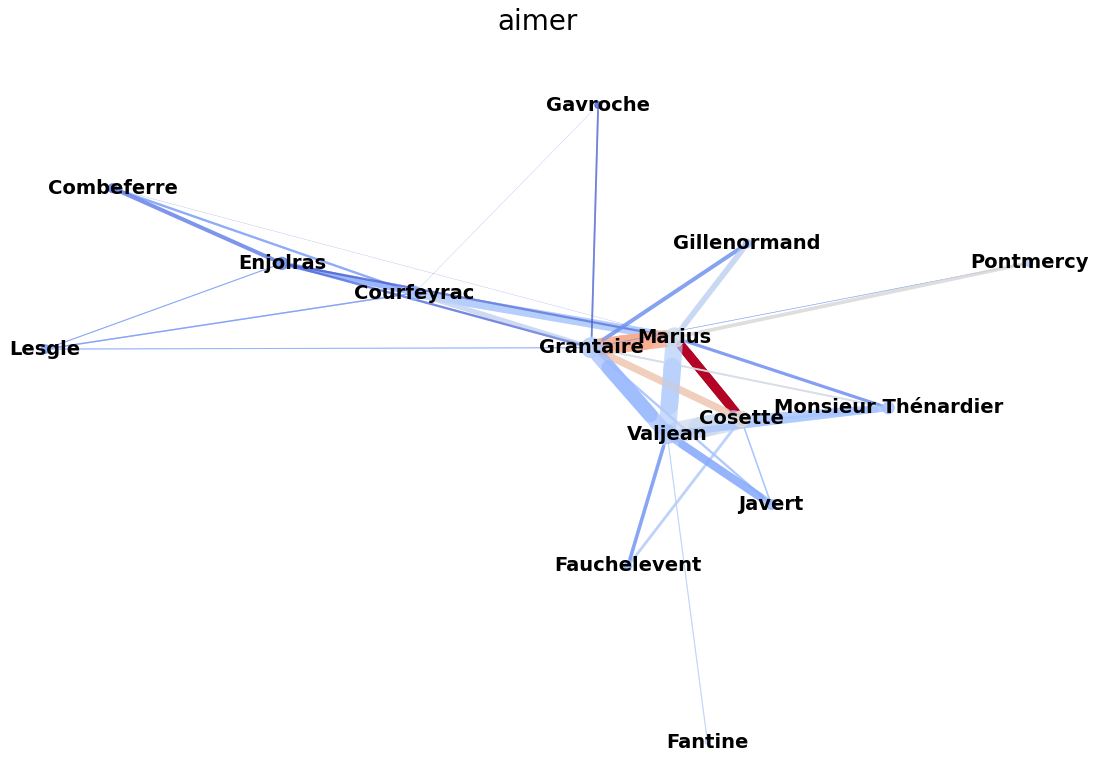
\includegraphics[width=0.45\textwidth]{fig/aimer.png} 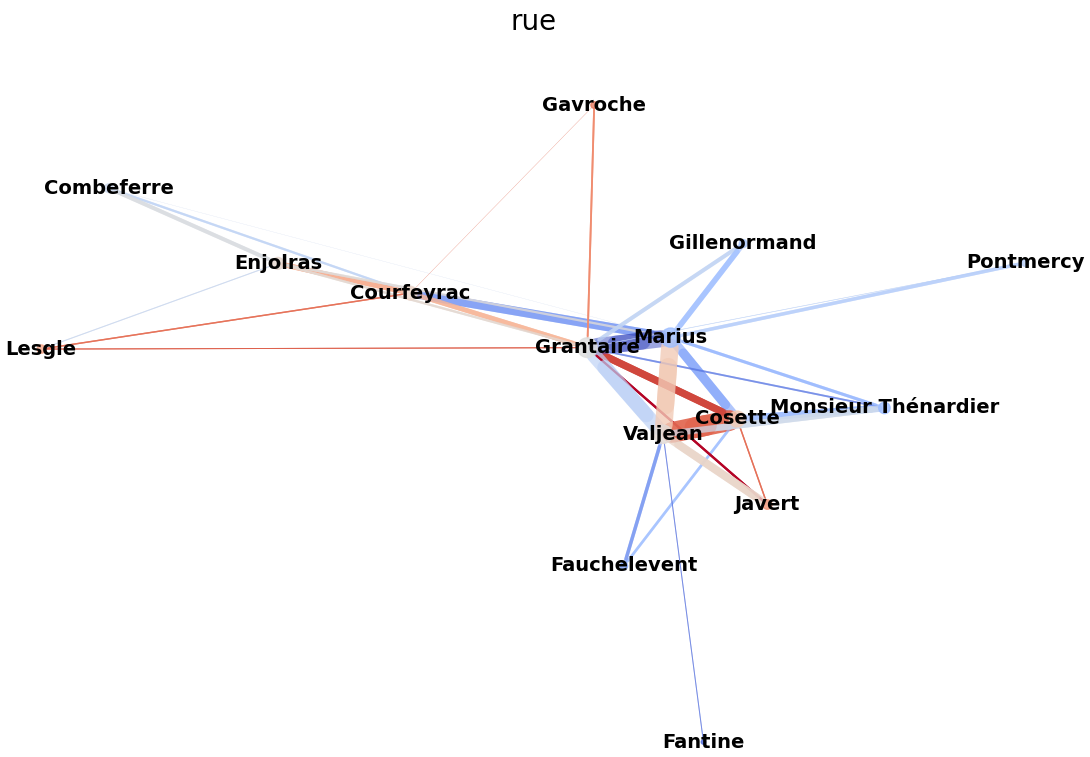
\includegraphics[width=0.45\textwidth]{fig/rue.png}
	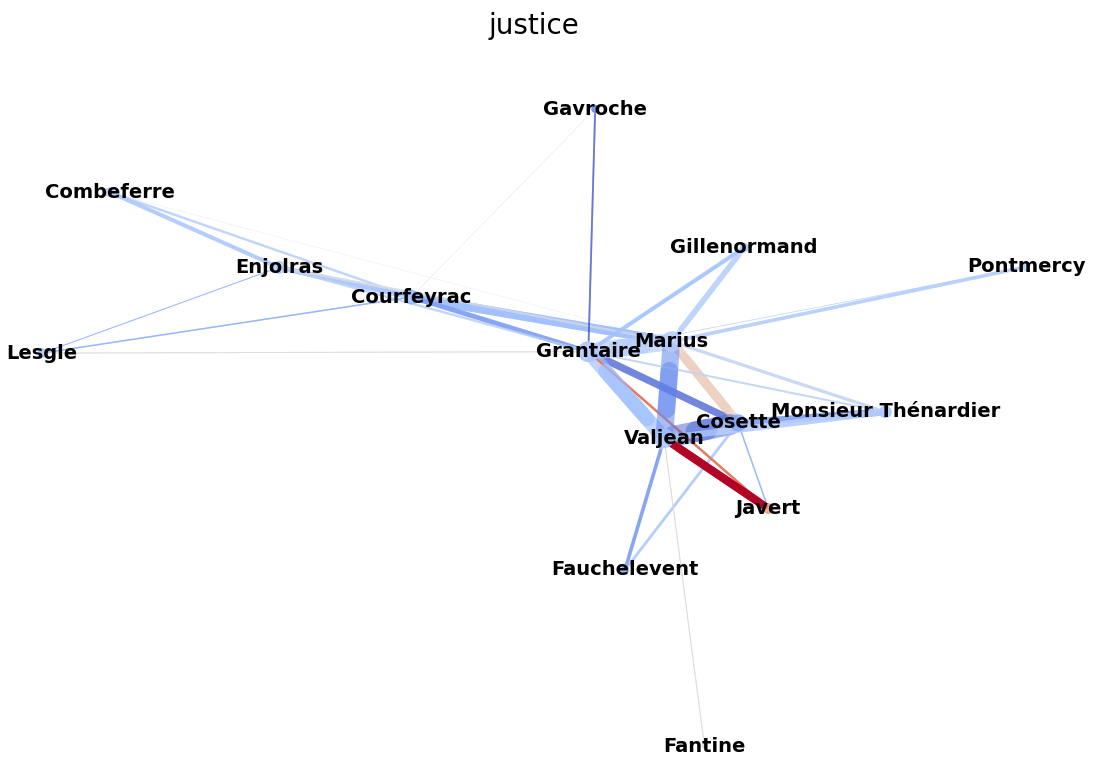
\includegraphics[width=0.45\textwidth]{fig/justice.png}
	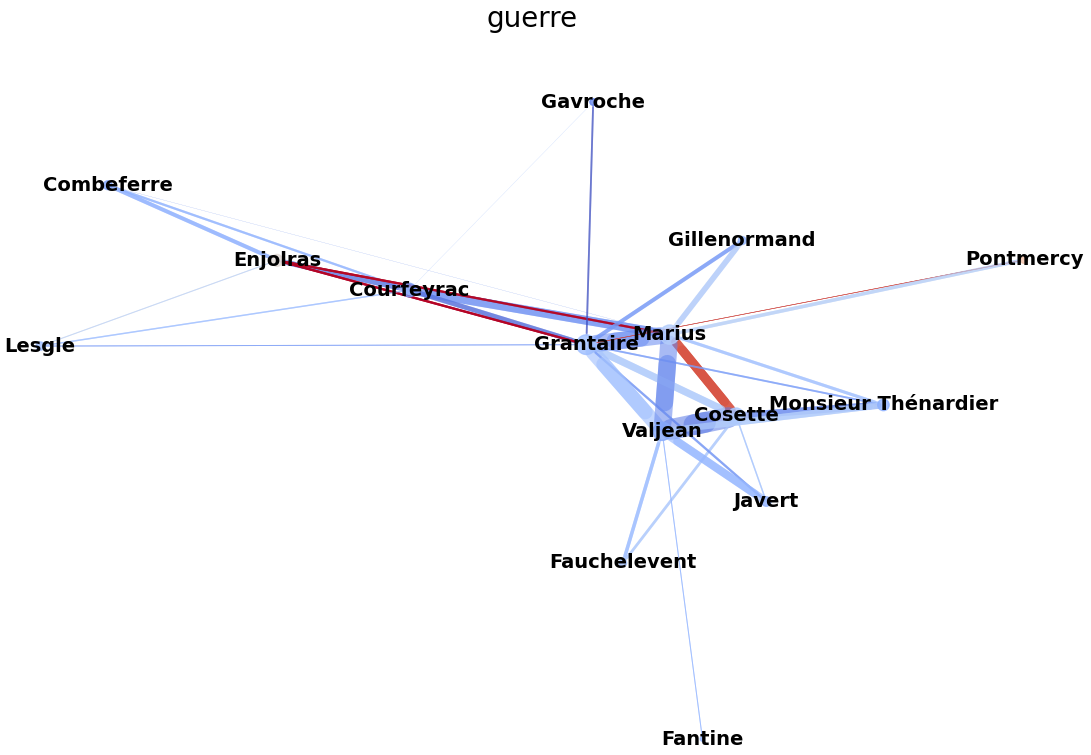
\includegraphics[width=0.45\textwidth]{fig/guerre.png}
	\label{networks}
	\caption{Resulting weighted and signed networks between main characters, with examples of word queries ("aimer", "rue", "justice", and "guerre"). These networks are computed with \textbf{CA-REG} method ($\lambda = 0.01$). Red indicate positive affinity, blue negative affinity, and edge width is proportional to the number of detected interactions between characters.}
\end{figure*}

%------------------------------

These results are extracted from the transposed table from the last, and display the most associated entities to a selected set of words. They can be found in Table 4. This type of results can be seen as queries, made from a single word, which output the most associated entities in the work related to that query. We chose here to show top entities related to words "aimer", "rue", "justice" and "guerre", as they represent some of the main topics of the book. In this task again, from our point of view, the \textbf{CA-REG} displays the most accurate results: the main love relationship (Cosette-Marius) of the book is the most associated entity for "aimer", several "amis de l'ABC" (a revolutionary group) are most associated with "rue", the cop-suspect relationship (Javert-Valjean) is the top entity for "justice", and military officers or bellicose characters are associated with "guerre". While somewhat inferior with the selected set of queries, \textbf{WV} methods have the advantage to be able to query words outside the scope of the book, as the pre-trained word embedding possess a very large vocabulary. It should also give interesting results when comparing different corpora, due to the fixed nature of word-vectors, but case studies concerning multiple corpora are outside the scope of this article.

Note that another way to represent these results is through weighted signed networks, as found in Figure 1 (for \textbf{CA-REG}). The network structure represent the number of time characters are detected together (which do not depend on the query), and the signed weights (edge color) display similarities between character relationship (edges) and the queried word. This representation gives a quick visual support in order to explore the studied work and could be implemented as a standalone program.


\subsubsection{A diachronic study of the most associated words for a subset of character-based objects}
\label{diachronic}

\begin{table*}[!h]
	\centering
	\begin{tabular}{|c|c|c|c|c|c|}
		\hline
		\parbox[t]{2mm}{\multirow{24}{*}{\rotatebox[origin=c]{90}{\textbf{CA-REG}}}} 
		& $V_1$ & $V_2$ & $V_3$ & $V_4$ & $V_5$ \\ 
		\cline{2-6}
		& huissier (1.4) & cuirassier (3.38) & gamin (1.92) & émeute (1.48) & sable (3.04) \\
		& hôte (1.11) & infanterie (2.9) & mine (1.38) & révolte (0.86) & berge (2.32) \\
		& arras (0.92) & sacrement (2.69) & farce (0.81) & bourgeoisie (0.84) & égout (2.16) \\
		& lampe (0.91) & brigade (2.41) & ignorance (0.74) & populaire (0.82) & voûte (1.9) \\
		& montreuil (0.81) & division (2.4) & jondrette (0.7) & insurrection (0.81) & vase (1.89) \\ 
		\cline{2-6}
		& Valjean 1 & Valjean 2 & Valjean 3 & Valjean 4 & Valjean 5 \\ 
		\cline{2-6}
		& chandelier (1.03) & pelle (2.6) & ursule (1.49) & réverbère (0.98) & matelas (2.54) \\ 
		& toulon (0.8) & fossoyeur (2.35) & luxembourg (1.06) & hausser (0.45) & ronde (1.96) \\
		& gervai (0.73) & pioche (1.51) & tableau (0.93) & promenade (0.37) & galerie (1.06) \\ 
		& bagne (0.65) & carte (1.39) & banc (0.81) & lanterne (0.36) & lanterne (0.99) \\ 
		& maire (0.57) & mestienne (1.35) & mouchoir (0.77) & tuyau (0.35) & rive (0.99) \\ 
		\cline{2-6}
		& Cosette 1 & Cosette 2 & Cosette 3 & Cosette 4 & Cosette 5 \\ 
		\cline{2-6}
		& gargote (0.59) & seau (1.48) & - & ravissant (1.11) & encre (0.76) \\ 
		& balayer (0.57) & poupée (0.99) & - & céleste (0.76) & plume (0.59) \\
		& alouette (0.56) & source (0.84) & - & volupté (0.67) & noce (0.49) \\
		& servante (0.43) & gargote (0.71) & - & frémir (0.64) & chandelier (0.48) \\
		& mois (0.34) & mestienne (0.64) & - & lancier (0.6) & antichambre (0.47) \\
		\cline{2-6}
		& Cosette-Valjean 1 & Cosette-Valjean 2 & Cosette-Valjean 3 & Cosette-Valjean 4 & Cosette-Valjean 5 \\
		\cline{2-6}
		& maladie (0.49) & façade (0.68) & - & promenade (0.5) & noce (1.27) \\ 
		& médecin (0.48) & corbillard (0.66) & - & chaîne (0.47) & marié (0.93) \\
		& demain (0.33) & mestienne (0.6) & - & blessure (0.46) & mardi (0.89) \\
		& surprise (0.28) & bâtiment (0.56) & - & tuyau (0.45) & mariage (0.86) \\
		& auprès (0.28) & cul (0.55) &- & luxembourg (0.44) & file (0.65) \\ 
		\hline
		\hline
		\parbox[t]{2mm}{\multirow{24}{*}{\rotatebox[origin=c]{90}{\textbf{WV-REG}}}} 
		& $V_1$ & $V_2$ & $V_3$ & $V_4$ & $V_5$ \\ 
		\cline{2-6}
		& demander (0.36) & saint (0.39) & gamin (0.45) & violence (0.44) & égout (0.52) \\ 
		& décider (0.3) & mont (0.39) & garçon (0.42) & haine (0.42) & quai (0.45) \\ 
		& aider (0.3) & régiment (0.38) & jeune (0.36) & révolte (0.42) & rue (0.44) \\ 
		& expliquer (0.29) & chapelle (0.38) & enfant (0.35) & souffrance (0.4) & eau (0.42) \\
		& plaindre (0.29) & infanterie (0.36) & père (0.34) & étincelle (0.39) & chaussée (0.42) \\
		\cline{2-6}
		& Valjean 1 & Valjean 2 & Valjean 3 & Valjean 4 & Valjean 5 \\ 
		\cline{2-6}
		& essayer (0.29) & jean (0.54) & admirer (0.32) & jean (0.71) & jean (0.72) \\ 
		& réfléchir (0.27) & jacques (0.33) & passer (0.31) & jacques (0.41) & pantalon (0.42) \\ 
		& expliquer (0.24) & pantalon (0.29) & observer (0.3) & pantalon (0.36) & jacques (0.39) \\ 
		& agir (0.24) & mr (0.28) & guetter (0.3) & louis (0.34) & philippe (0.34) \\ 
		& questionner (0.24) & denis (0.28) & croiser (0.3) & philippe (0.33) & denis (0.33) \\ 
		\cline{2-6}
		& Cosette 1 & Cosette 2 & Cosette 3 & Cosette 4 & Cosette 5 \\ 
		\cline{2-6}
		& an (0.41) & dormir (0.33) & - & rêver (0.32) & rêver (0.31) \\
		& mois (0.39) & regarder (0.29) & - & regarder (0.31) & mentir (0.29) \\
		& mère (0.36) & sentir (0.28) & - & contempler (0.28) & écrire (0.29) \\
		& fille (0.35) & endormir (0.28) & - & pleurer (0.27) & demander (0.28) \\
		& enfant (0.33) & respirer (0.28) & - & lire (0.27) & pleurer (0.28) \\
		\cline{2-6}
		& Cosette-Valjean 1 & Cosette-Valjean 2 & Cosette-Valjean 3 & Cosette-Valjean 4 & Cosette-Valjean 5 \\
		\cline{2-6}
		& voir (0.32) & rue (0.55) & - & jean (0.52) & mariage (0.42) \\ 
		& entendre (0.31) & ruelle (0.48) & - & pantalon (0.35) & marié (0.4) \\ 
		& frissonner (0.3) & boulevard (0.45) & - & gilet (0.28) & noce (0.4) \\ 
		& grommeler (0.3) & mur (0.4) & - & gris (0.27) & gai (0.33) \\ 
		& essayer (0.3) & faubourg (0.4) & - & manteau (0.26) & amour (0.3) \\ 
		\hline
	\end{tabular}
	\label{TIME_REG_word_vs_obj}
	\caption{The 5 most associated words (similarity in parentheses) vs volumes constant, Valjen, Cosette, and Cosette-Valjean entity, as found in each tome regarding the \textbf{CA-REG} and \textbf{WV-REG} methods ($\lambda = 0.01$). Note that Cosette was not found in volume 3 because she is not explicitly cited (she is often refereed as "the daugther of M. Leblanc").}
\end{table*}

These results are obtained from the table $\mathbf{O}_\text{vol}$ where entities are considered different based on the volume. By doing so, it permits to track, e.g., the evolution of associated words for entities along the book. Moreover, we also define a constant term $V_i$ for each volumes $i$, which absorbs the associated words for each volume. Results for constants and a subset of entities can be found in Table 5. Note that we did not show \textbf{CONT} results in this table, as they are similar to the one found in Table 3 : words are often repeated themselves among object. 

Here again, we see that associated words for the \textbf{WV} method are less specific and again give the general tone of the tome or entity. 

\section{Conclusion}

\appendix

\section{Appendix}

\subsection{Correspondence Analysis}
\label{ca_details}

Starting from the $(n \times v)$ contingency table $\mathbf{N} = (n_{ij})$, we define the vector of unit weights as $\mathbf{f} = (f_i) := (n_{i\bullet}/n_{\bullet \bullet})$ and the vector of word weights as $\mathbf{g} = (g_j) := (n_{\bullet j}/n_{\bullet \bullet})$, where $\bullet$ denotes the summation on the replaced index. It is then possible to compute the \emph{weighted scalar product matrix between units} $\mathbf{K} = (k_{ij})$ with

\begin{equation}
k_{ij} := \sqrt{f_i f_j} \sum_{k=1}^{v} g_k(q_{ik} - 1)(q_{jk} - 1), 
\end{equation}

where $q_{ik} = \frac{n_{ik} n_{\bullet \bullet}}{n_{j \bullet} n_{\bullet k}}$ is the \emph{quotient of independence} of the cell $i, k$. The vector of textual unit $i$, $\mathbf{x}_i = (x_{i\alpha})$, is obtained by the eigendecomposition of the matrix $\mathbf{K} = \mathbf{U}\bm{\Lambda}\mathbf{U}^\top$ and with

\begin{equation}
x_{i\alpha} := \frac{\sqrt{\lambda_\alpha}}{\sqrt{f_i}} u_{i \alpha},
\end{equation}

where $\lambda_\alpha$ are the eigenvalues contained in the diagonal matrix $\bm{\Lambda}$ and $u_{i \alpha}$ the eigenvectors components found in $\mathbf{U}$. We find the vector of word $j$, $\mathbf{w}_j = (w_{j\alpha})$, with 

\begin{equation}
w_{j\alpha} := \frac{1}{\sqrt{\lambda_\alpha}} \sum_{i=1}^v f_i q_{ij} x_{i \alpha}.
\end{equation}

Note that various other quantities of interest can also be computed in CA, such as 
\begin{align*}
p_\alpha &:= \frac{\lambda_\alpha}{\lambda_\bullet} :\text{\small the proportion of inertia expressed in $\alpha$,} \\
c^u_{i \alpha} &:= \frac{f_i x_{i\alpha}^2}{\lambda_\alpha} : \text{\small the contribution of unit $i$ to axis $\alpha$,} \\
c^w_{j \alpha} &:= \frac{g_j w_{j\alpha}^2}{\lambda_\alpha} : \text{\small the contribution of word $j$ to axis $\alpha$,} \\
h^u_{i \alpha} &:= \frac{x_{i\alpha}^2}{\sum_{\alpha} x_{i\alpha}^2} : \text{\small the contribution of  axis $\alpha$ to unit $i$,} \\
h^w_{j \alpha} &:= \frac{w_{j\alpha}^2}{\sum_{\alpha} w_{j\alpha}^2} : \text{\small the contribution of  axis $\alpha$ to word $j$,}
\end{align*}
For a detailed interpretation of these different quantities, see (REF). 

\subsection{Unit embedding based of pre-trained word vectors}
\label{wv_details}

This methods is justified and detailed in (REF). Let $\mathbf{w}_1, \ldots, \mathbf{w}_v$ be pre-trained word vectors which appear in the studied corpus, and the $(n \times v)$ table $\mathbf{N}$ counting the frequency of these words in the $n$ textual units. We first construct the \emph{uncentered vectors} $\widetilde{\mathbf{x}}_i$ of each unit $i$ with
\begin{equation}
\widetilde{\mathbf{x}}_i = \sum_{j = 1}^v \frac{n_{ij}}{n_{i \bullet}} \frac{a}{a + \frac{n_{\bullet j}}{n_{\bullet \bullet}}} \mathbf{w}_j,
\end{equation}
where $a > 0$ is an hyperparameter which gives less importance to frequent words as $a \to 0$. In this article, we set $a$ to the recommended value of $0.01$. Let $\widetilde{\mathbf{X}}$ be the matrix whose columns are vectors $\widetilde{\mathbf{x}}_i$, and $\mathbf{u}$ be its first singular vector. We compute \emph{vectors} $\mathbf{x}_i$ of each units $i$ with
\begin{equation}
\mathbf{x}_i = \widetilde{\mathbf{x}}_i - \mathbf{u}\mathbf{u}^\top \widetilde{\mathbf{x}}_i.
\end{equation}
This last equation act like a \emph{centration} of unit vectors in the direction of the first singular vector $\mathbf{u}$.

%% Define the bibliography file to be used
\bibliography{charnet}

\end{document}

%%
%% End of file
